\section{Results and Discussion}
\subsection{Six DOF Stewart Platform}
As earlier mentioned, the Stewart platform has already been designed and fabricated and our part in this work was to do an evaluation of the same to verify its mechanical feasibility. As such, the various parts of the platform were obtained and assembled. For further analysis, a 3D model of the same platform was done using Autodesk Inventor.

The assembled Stewart platform is as shown in figure \ref{fig}. Figure \ref{fig1} shows the Stewart platform configuration setup with the Wind tunnel's test section.
\begin{center}
	\begin{figure}[H]
		\centering
		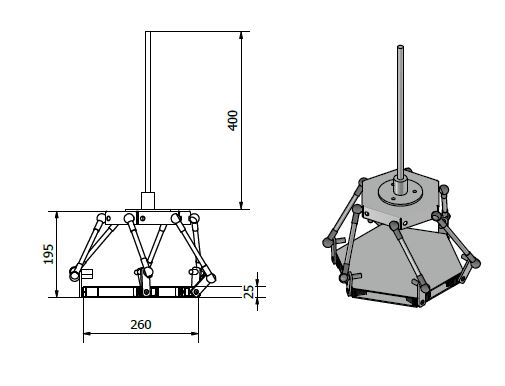
\includegraphics[width=1\linewidth]{Figures/Assembly.JPG}
		\caption[Assembled Platform]{Assembly of Stewart Platform}
		\label{fig}
	\end{figure}
\end{center}
\begin{figure}[!htb]%
	\centering
	\subfloat[\centering Design]{{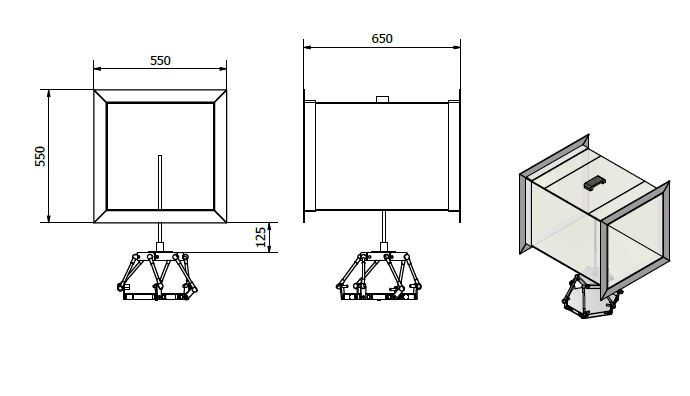
\includegraphics[width=8cm]{Figures/Test-section.JPG} }}%
	\qquad
	\subfloat[\centering Model placement in test section]{{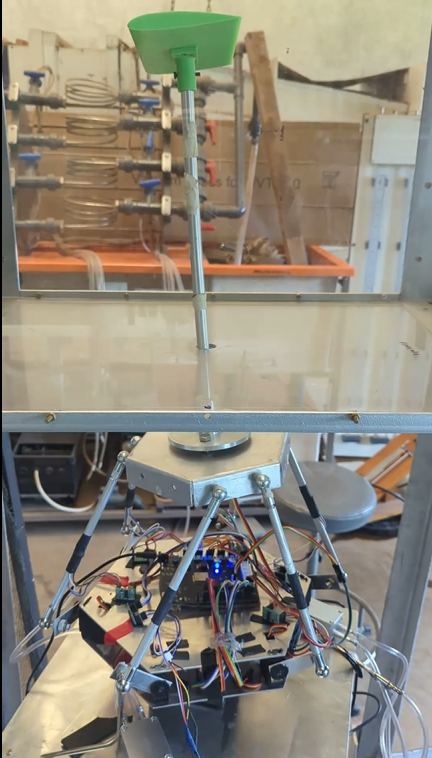
\includegraphics[width=3cm]{Figures/stew_wind1.png}}}
	\caption[Stewart Platform and Test Section]{Stewart platform and Test section configuration}%
	\label{fig:result}%
\end{figure}

\subsection{Strut}
Computational Fluid Dynamics was done for various values of air speed and the following drag forces were
determined from the simulations.
\begin{table}[H]
	\caption{CFD Results}
	\end{table}
	\begin{center}
	\begin{tabular}{|l|l|}
	\hline
	\textbf{Air Velocity(m/s)} & \textbf{Drag Force (N)}\\
	\hline
	10 & 1.203 \\
	\hline
	10 & 6.838 \\
	\hline
	30 & 8.068 \\
	\hline
	40 & 11.367 \\
	\hline
	\end{tabular}
\end{center}
Figure \ref{cfd} shows the effect of the strut to air flow.
\begin{center}
	\begin{figure}[H]
		\centering
		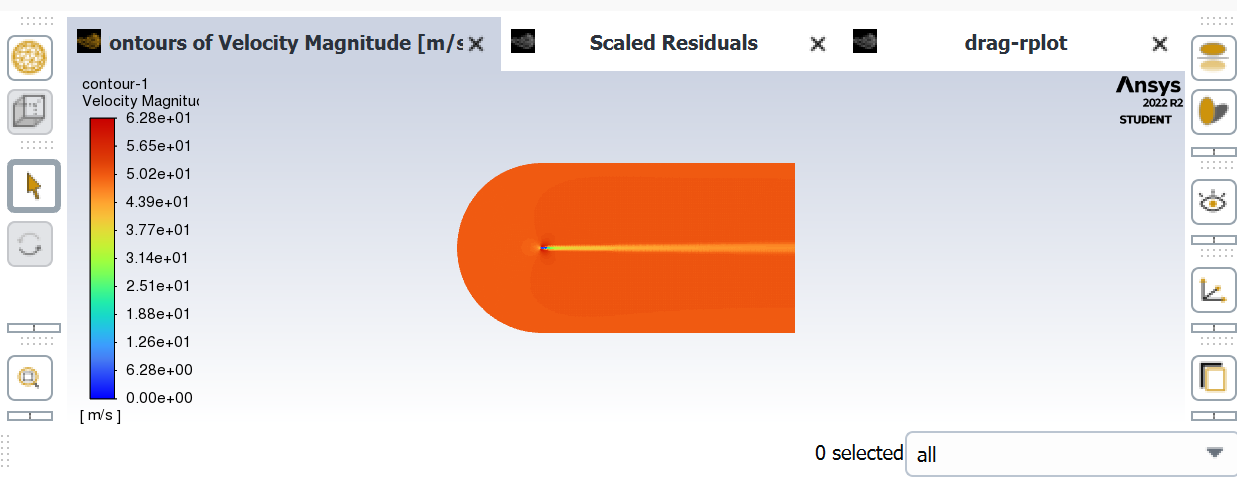
\includegraphics[width=0.8\linewidth]{Figures/CFD.png}
		\caption[CFD]{Computational Fluid Dynamics showing the effect of the strut to air flow}
		\label{cfd}
	\end{figure}
\end{center}

\subsection{Force Measurement by the Stewart Platform}
A static analysis test was performed and the following results were obtained:
\begin{table}[H]
	\caption{FEA Results}
\end{table}
\begin{center}
	\begin{tabular}{|l|l|l|}
		\hline
		\textbf{Name}     & \textbf{Minimum} & \textbf{Maximum} \\
		\hline
		Von Mise's        & 0 MPa            & 63.19 MPa        \\
		\hline
		Displacement      & 0 mm             & 23.74 mm         \\
		\hline
		Safety Factor     & 10.3426 ul       & 15 ul            \\
		\hline
		Equivalent Strain & 0 ul             & 0.052 ul         \\
		\hline
	\end{tabular}
\end{center}
Finite Element Analysis done showed expected strain values on each
Stewart platform leg as shown in figure \ref{strain1}.

\begin{center}
	\begin{figure}[H]
		\centering
		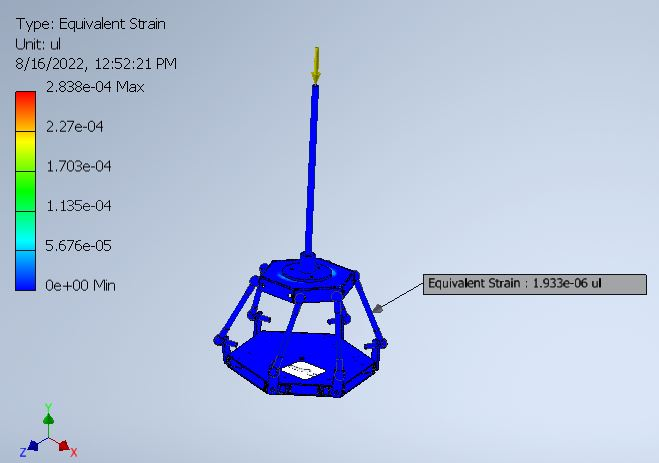
\includegraphics[width=0.6\linewidth]{Figures/Equivalent}
		\caption[Equivalent strain]{Strain induced on each of the legs}
		\label{strain1}
	\end{figure}
\end{center}
These strains are small and undergo amplification in order provide substantial input for the strain gauges used for force measurements.

\subsection{Human Machine Interface}
The user interface of the platform was programmed using golang and this resulted in the view below with the use of sliders for platform positioning and buttons to set model orientations and start data collection.
\begin{center}
	\begin{figure}[H]
		\centering
		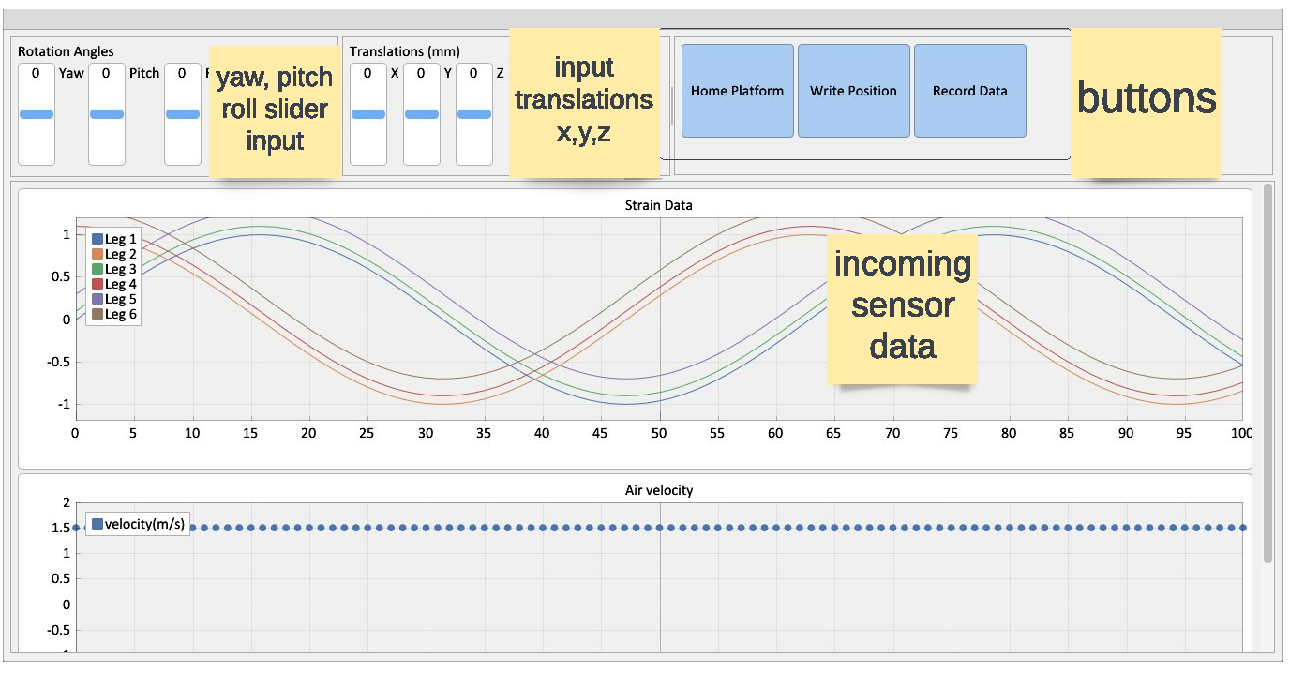
\includegraphics[width=1\linewidth]{Figures/hmi}
		\caption[HMI Dashboard]{HMI Dashboard}
	\end{figure}
\end{center}

The top bar of the user interface includes slider buttons to control platform orientation and commands around recording data and calibration as shown in figure \ref{fig:hmi_top}.
\begin{center}
	\begin{figure}[H]
		\centering
		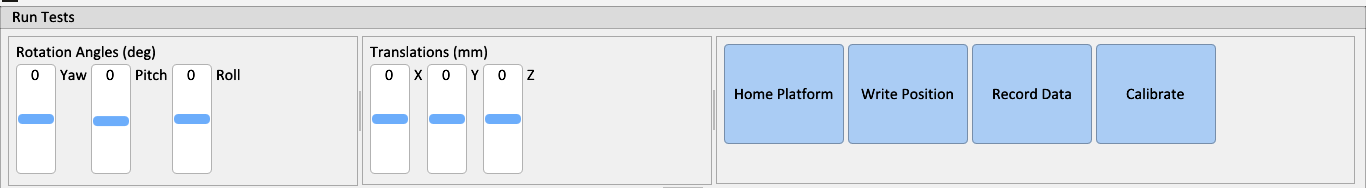
\includegraphics[width=1\linewidth]{Figures/Screenshot 2022-12-11 195125.png}
		\caption[HMI Top Bar]{HMI Top Bar}
		\label{fig:hmi_top}
	\end{figure}
\end{center}

The menu bar also provides options to test the six degrees of freedom for the whole platform as shown in figure \ref{fig:hmi_menu}.
\begin{center}
	\begin{figure}[H]
		\centering
		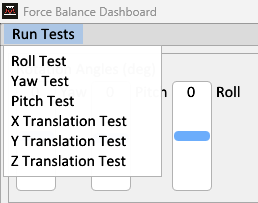
\includegraphics{Figures/Screenshot 2022-12-11 195108.png}
		\caption[HMI menubar]{HMI menubar}
		\label{fig:hmi_menu}
	\end{figure}
\end{center}
A calibration window is also included that is used to set the calibration factor for measurements taken as shown in figure \ref{fig:hmi_calib}
\begin{center}
	\begin{figure}[H]
		\centering
		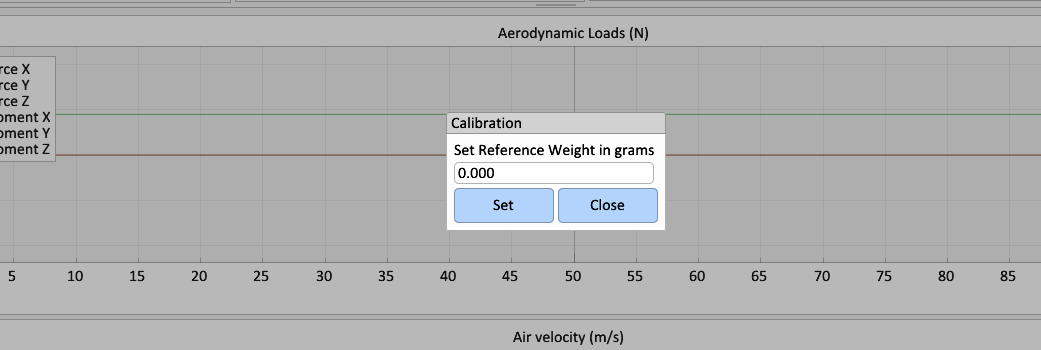
\includegraphics[width=1\linewidth]{Figures/Screenshot 2022-12-11 195034.png}
		\caption[HMI calibration]{HMI calibration}
		\label{fig:hmi_calib}
	\end{figure}
\end{center}
The incoming sensor data was also displayed on the screen as shown in the following figures:
\begin{center}
	\begin{figure}[H]
		\centering
		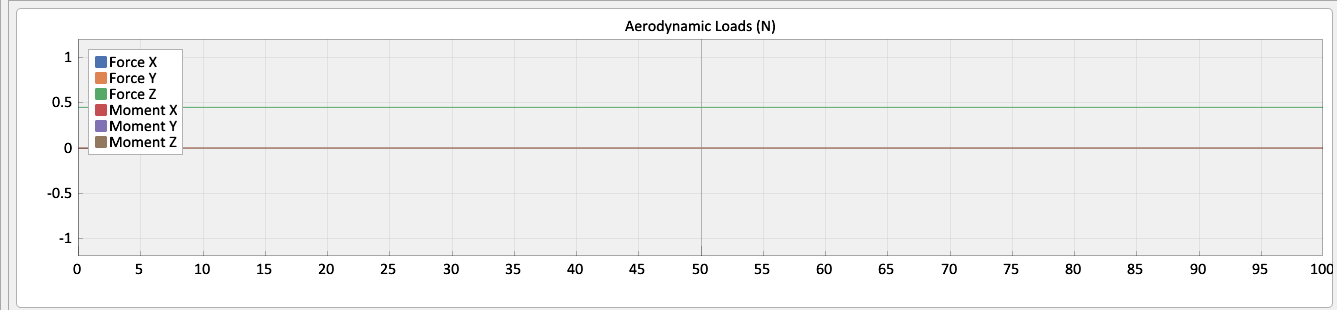
\includegraphics[width=1\linewidth]{Figures/Screenshot 2022-12-11 194656.png}
		\caption[HMI Aerodynamic loads]{HMI Aerodynamic loads}
	\end{figure}
\end{center}
\begin{center}
	\begin{figure}[H]
		\centering
		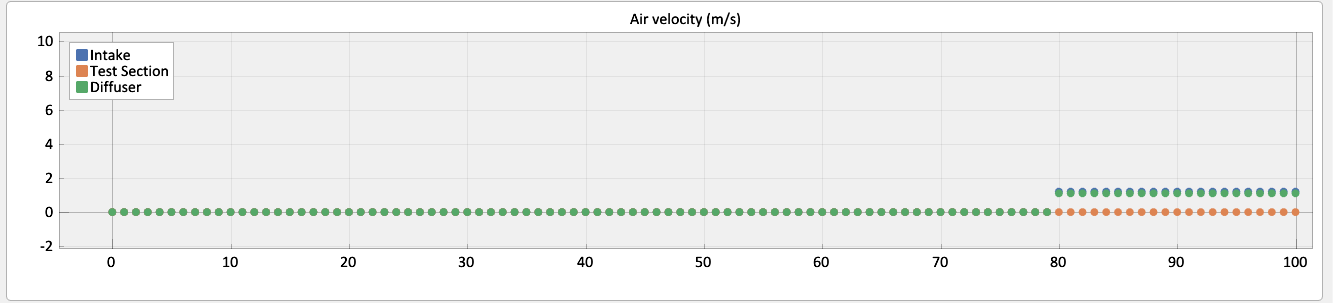
\includegraphics[width=1\linewidth]{Figures/Screenshot 2022-12-11 194826.png}
		\caption[HMI Air velocity]{HMI Air velocity}
	\end{figure}
\end{center}
\begin{center}
	\begin{figure}[H]
		\centering
		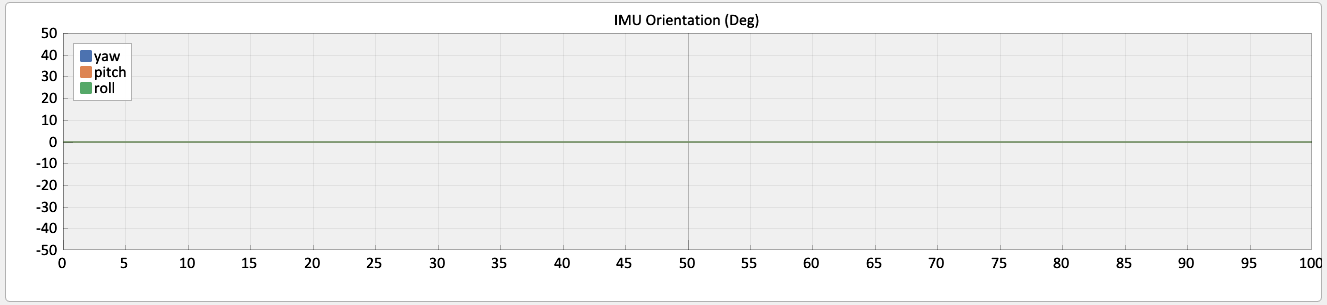
\includegraphics[width=1\linewidth]{Figures/Screenshot 2022-12-11 194952.png}
		\caption[HMI IMU readings]{HMI IMU readings}
	\end{figure}
\end{center}
\begin{center}
	\begin{figure}[H]
		\centering
		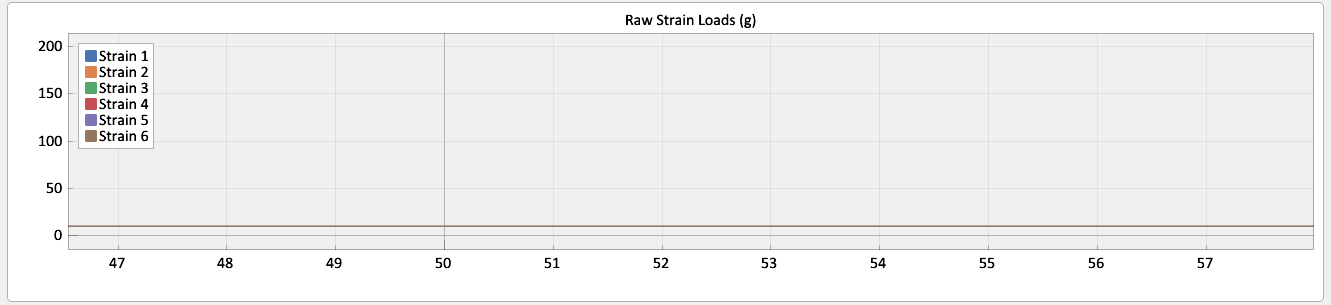
\includegraphics[width=1\linewidth]{Figures/Screenshot 2022-12-11 194931.png}
		\caption[HMI Raw Strain]{HMI Raw Strain}
	\end{figure}
\end{center}
\subsection{PCB}
The schematics from the electrical designs as seen in the appendix were routed to generate a PCB ready for manufacture. The fabricated PCB is shown in figure \ref{fig:pcb_fab}
\begin{center}
	\begin{figure}[H]
		\centering
		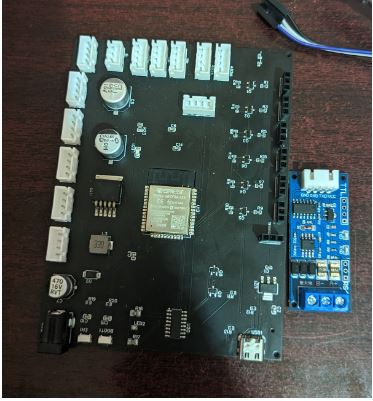
\includegraphics[width=0.7\linewidth]{Figures/pcb 1.JPG}
		\caption[Printed Circuit Board view]{Printed Circuit Board}
		\label{fig:pcb_fab}
	\end{figure}
\end{center}
The PCB is compact as shown in the figure \ref{fig:pcb_fab}. It is also integrates most of the components to minimize use of wires to make connections.

\subsection{Smoke Visualization}
\subsubsection{Smoke Rake}
The smoke rake was 3D printed at iPIC and assembled with its lid as shown.
\begin{figure}[!htb]%
	\centering
	\subfloat[\centering Smoke Rake CAD]{{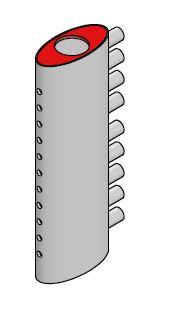
\includegraphics[width=3cm]{Figures/Rake CAD.JPG} }}%
	\qquad
	\subfloat[\centering 3D Printed Rake]{{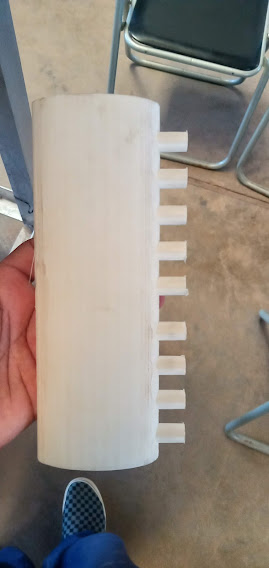
\includegraphics[width=3cm]{Figures/smoke emitter.jpg}}}
	\caption[3D Printed rake]{Smoke rake and lid assembled}%
	\label{fig:result}%
\end{figure}
\subsubsection{Smoke Rake and Pipe Assembly}
The Smoke rake was assembled with a metal pipe for rigid support and also for smoke introduction into the
smoke rake as shown.
\begin{figure}[!htb]%
	\centering
	\subfloat[\centering CAD Assembly]{{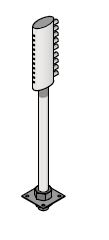
\includegraphics[width=3cm]{Figures/CAD assembly.JPG} }}%
	\qquad
	\subfloat[\centering Final Part]{{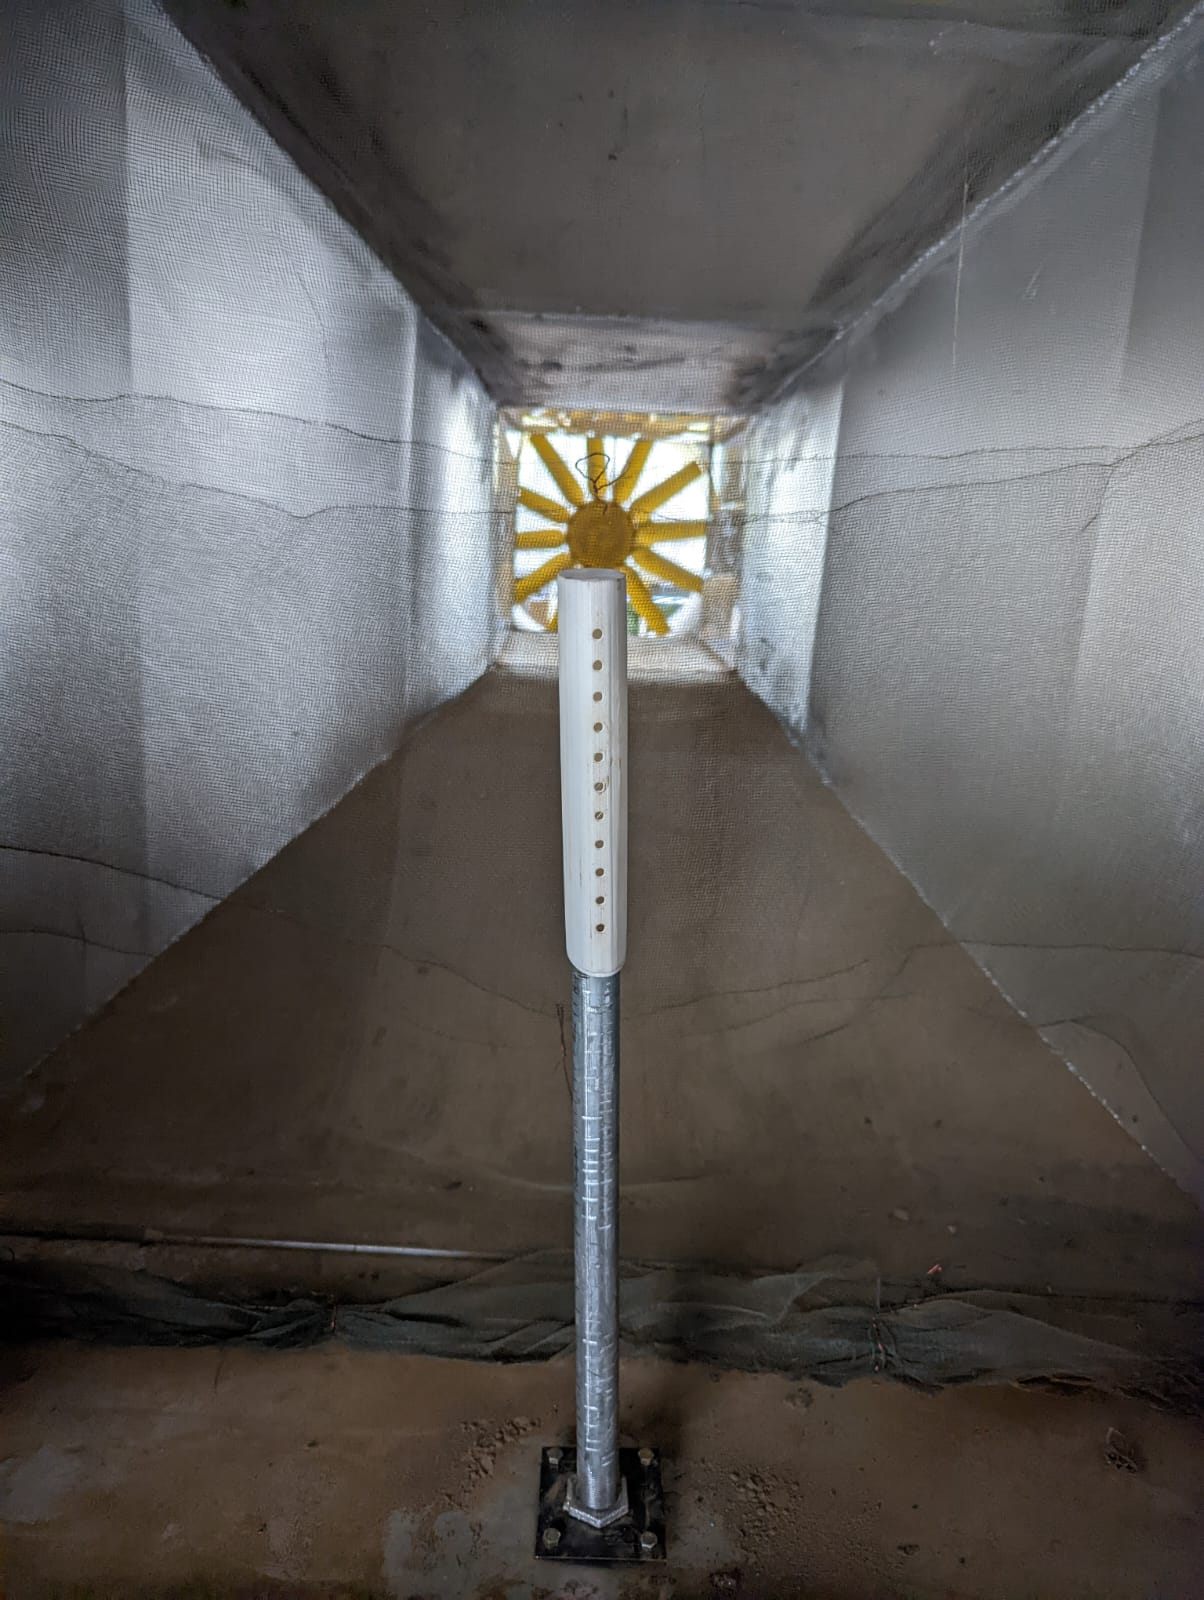
\includegraphics[width=4.5cm]{Figures/final pipe.jpg}}}
	\caption[Final rake and pipe]{Smoke rake and pipe assembly and setup in the wind tunnel}%
	\label{fig:result1}%
\end{figure}

\subsection{Discussion}
The Stewart platform is able to position models in various dynamic positions depending on the angle values
of yaw, roll and pitch as well as the amount of displacements in the x-, y- and z-directions input via the HMI.
 Application of load on the platform
subjects each of the legs to axial forces which causes strain. This strain can be used to determine aerodynamic forces
on models during wind tunnel testing. However, aerodynamic forces due to the strut must be put to account because from
simulations, drag forces are developed by the strut when there is airflow. Smoke introduced into the wind tunnel allows
visualization of airflow around a model. Pitot tube probes used and their transducers provide valuable information used 
in post analysis to determine the aerodynamic coefficients (drag, lift).